\input{E:/Blaok/Works/LaTeX/MATLAB.tex}

\begin{document}
\title{语音合成大作业}
\author{池雨泽}
\maketitle
\section{}
\noindent\ding{125}{\CJKfamily{kai}给定$$e(n) = s(n)-a_1s(n-1)-a_2s(n-2)$$假设e(n)是输入信号,s(n) 是输出信号,上述滤波器的传递函数是什么?如果$a1 = 1.3789$,$a2 = -0.9506$ ,上述合成模型的共振峰频率是多少?用zplane ,freqz ,impz 分别绘出零极点图,频率响应和单位样值响应。用filter 绘出单位样值响应,比较和impz 的是否相同。}\ding{126}
\par
传递函数即$$H(z)=\frac{1}{1-a_1 z^{-1}-a_2 z^{-2}}.$$共振峰频率为$0.1250\times \mbox{采样率}$。假设采样率为8kHz,则共振峰频率为1kHz。\newline
零极点图\begin{center}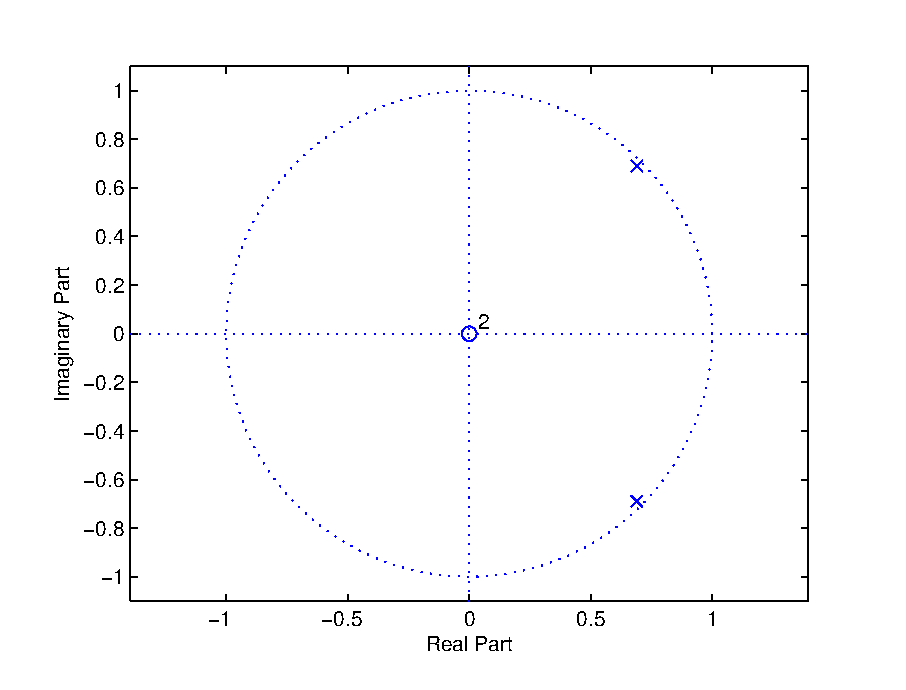
\includegraphics[width=\textwidth]{A2_1_zplane.eps}\end{center}
频率响应\begin{center}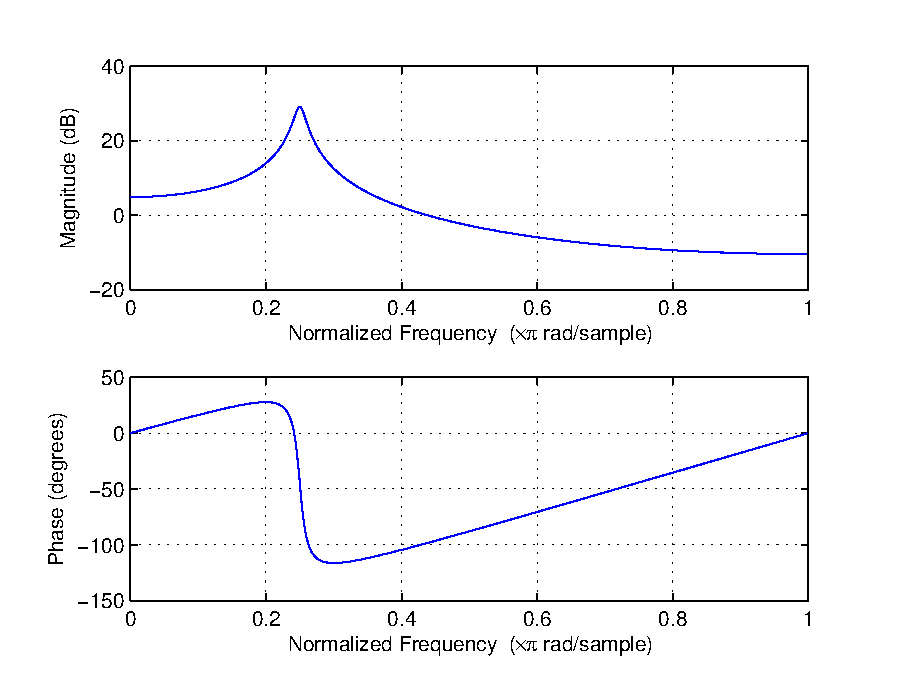
\includegraphics[width=\textwidth]{A2_1_freqz.eps}\end{center}
impz绘制的单位样值响应\begin{center}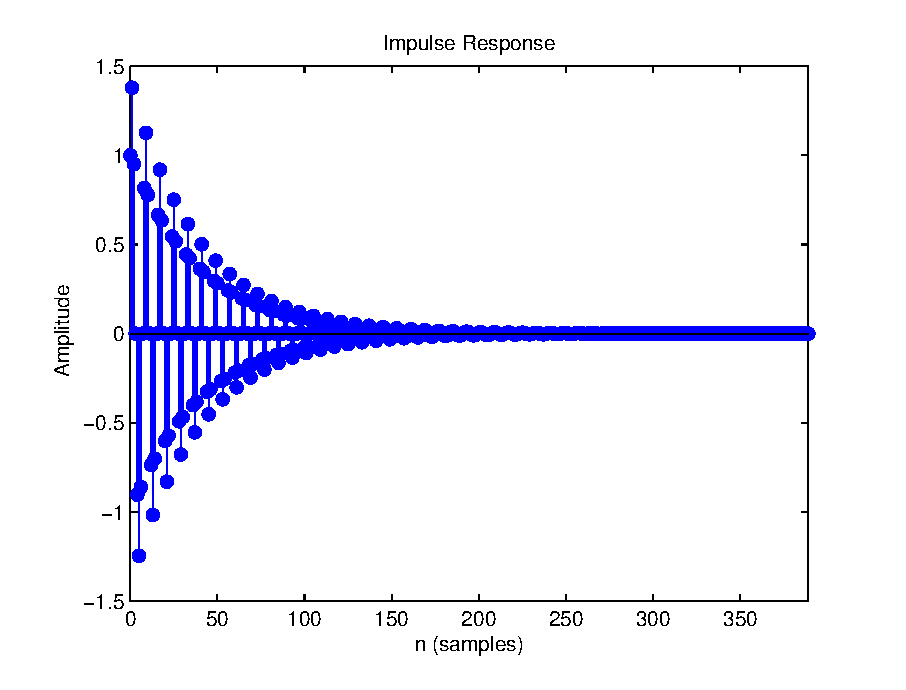
\includegraphics[width=\textwidth]{A2_1_impz.eps}\end{center}
filter绘制的单位样值响应\begin{center}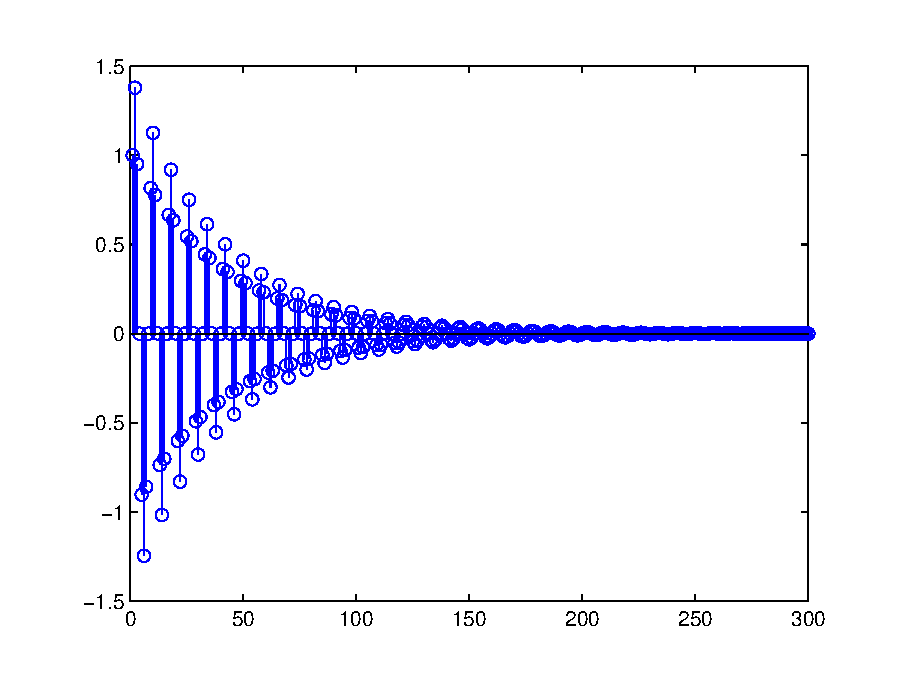
\includegraphics[width=\textwidth]{A2_1_filter.eps}\end{center}
可见二者完全相同。
\section{}
\noindent\ding{125}{\CJKfamily{kai}阅读speechproc.m 程序,理解基本流程。程序中已经完成了语音分帧、加窗、线性预测、和基音周期提取等功能。注意:不要求掌握线性预测和基音周期提取的算法原理。}\ding{126}
\par
假定采样率为8kHz,每帧80个采样点即是10ms,窗长240则每次移动1/3窗长,前两帧不做处理,循环处理每一帧中的语音。
\section{}
\noindent\ding{125}{\CJKfamily{kai}运行该程序到27 帧时停住,用(1)中的方法观察零极点图。}\ding{126}
\par
\begin{center}\includegraphics[width=\textwidth]{A2_3.eps}\end{center}
\section{}
\noindent\ding{125}{\CJKfamily{kai}在循环中添加程序:对每帧语音信号$s(n)$ 和预测模型系数$\{a_i\}$,用filter 计算激励信号$e(n)$ 。注意:在系数变化的情况下连续滤波,需维持滤波器的状态不变,要利用filter 的zi 和zf 参数。}\ding{126}
\par
初始时滤波器状态为0,以后每次利用原有状态更新现有状态。
\section{}
\noindent\ding{125}{\CJKfamily{kai}完善speechproc.m 程序,在循环中添加程序:用你计算得到的激励信号$e(n)$ 和预测模型系数$\{a_i\}$ ,用filter 计算重建语音$\hat{s}(n)$ 。同样要注意维持滤波器的状态不变。}\ding{126}
\par
与上一问类似,但要反过来用滤波器。
\section{}
\noindent\ding{125}{\CJKfamily{kai}在循环结束后添加程序:用sound 试听(6)中的$e(n)$ 信号,比较和$s(n)$ 以及$\hat{s}(n)$信号有何区别。对比画出三个信号,选择一小段,看看有何区别。}\ding{126}
\par
整个信号
\begin{center}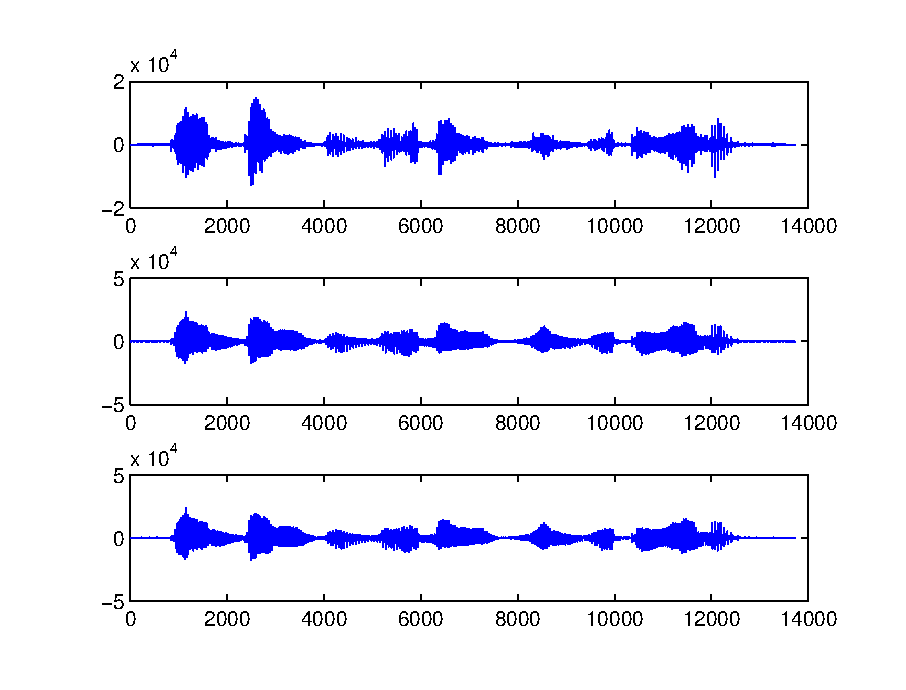
\includegraphics[width=\textwidth]{A2_6_whole.eps}\end{center}
其中5000-6000的细节
\begin{center}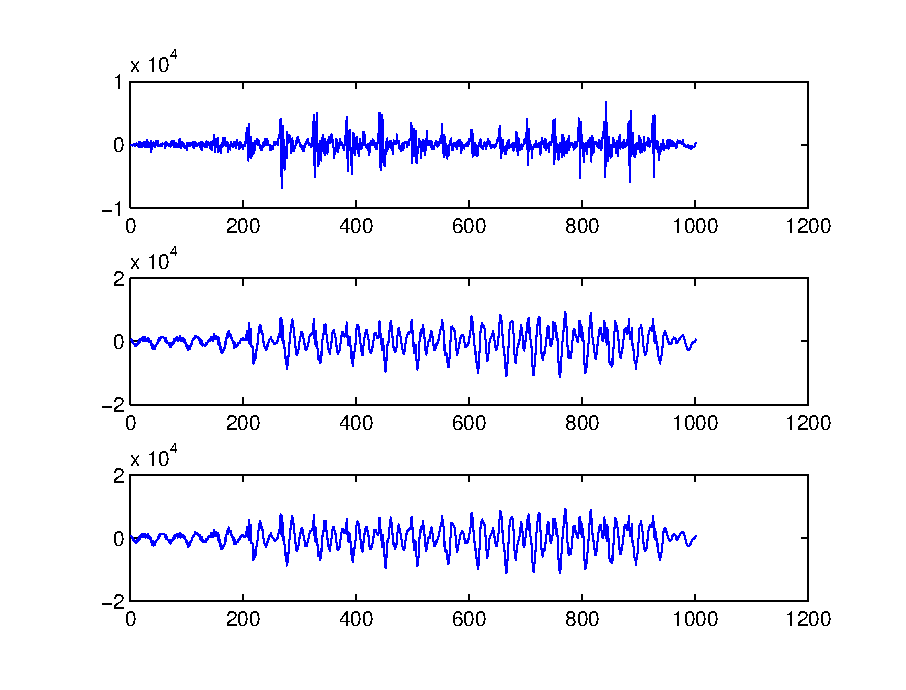
\includegraphics[width=\textwidth]{A2_6_detail.eps}\end{center}
$e(n)$与$s(n)$相差并不大,主要的差别在于$e(n)$具有频率更低的周期性,即基音周期。$e(n)$保留了$s(n)$的很多信息,可以听出语音,但噪声特别严重,这应当是基音周期带来的噪声。$s(n)$与$\hat{s}(n)$则几乎完全相同,相对误差(误差范数/范数)约为 0.0059,节选出来的部分相对误差更低至$10^{-16}$,听起来二者没有差异,均为有少许噪声的语音。
\section{}
\noindent\ding{125}{\CJKfamily{kai}生成一个8kHz 抽样的持续1 秒钟的数字信号,该信号是一个频率为200Hz 的单位样值“串”,即$$x(n)=\sum_{i=0}^{NS-1}\delta(n-iN)$$考虑该信号的N 和NS 分别为何值?用sound 试听这个声音信号。再生成一个300Hz 的单位样值“串”并试听,有何区别?事实上,这个信号将是后面要用到的以基音为周期的人工激励信号$e(n)$ 。}\ding{126}
\par
N=40,NS=200。300Hz信号听起来比200Hz音调更高。
\section{}
\noindent\ding{125}{\CJKfamily{kai}真实语音信号的基音周期总是随着时间变化的。我们首先将信号分成若干个10毫秒长的段,假设每个段内基音周期固定不变,但段和段之间则不同,具体为$$PT = 80 + 5mod(m, 50)$$其中PT 表示基音周期,m 表示段序号。生成1 秒钟的上述信号并试听。(提示:用循环逐段实现,控制相邻两个脉冲的间隔为其中某个脉冲所在段的PT值。)}\ding{126}
\par
是音调周期性变化的声音,有点类似喇叭声。
\section{}
\noindent\ding{125}{\CJKfamily{kai}用filter 将(8)中的激励信号$e(n)$ 输入到(1)的系统中计算输出$s(n)$ ,试听和$e(n)$ 有何区别。}\ding{126}
\par
处理后的声音感觉更厚重,发声物件有一定共鸣腔的感觉。
\section{}
\noindent\ding{125}{\CJKfamily{kai}重改speechproc.m 程序。利用每一帧已经计算得到的基音周期和(8)的方法,生成合成激励信号$Gx(n)$( G 是增益),用filter 函数将$Gx(n)$ 送入合成滤波器得到合成语音$\tilde{s}(n)$ 。试听和原始语音有何差别。}\ding{126}
\par
合成语音可以清楚地听出语言内容,但出现了少许原来没有的杂音。
\section{}
\noindent\ding{125}{\CJKfamily{kai}仿照(10)重改speechproc.m 程序,只不过将(10)中合成激励的长度增加一倍,即原来10 毫秒的一帧变成了20 毫秒一帧,再用同样的方法合成出语音来,如果你用原始抽样速度进行播放,就会听到慢了一倍的语音,但是音调基本没有变化。}\ding{126}
\par
这时得到的语音时长为原来的二倍,但音调基本与原来一致,这与直接resample得到的结果完全不同。
\section{}
\noindent\ding{125}{\CJKfamily{kai}重新考察(1)中的系统,将其共振峰频率提高150Hz 后的$a_1$ 和$a_2$ 分别是多少?}\ding{126}
\par
$a_1=1.2073,a_2=-0.9506.$
\section{}
\noindent\ding{125}{\CJKfamily{kai}仿照(10)重改speechproc.m 程序,但要将基音周期减小一半,将所有的共振峰频率都增加150Hz ,重新合成语音,听听是何感受。}\ding{126}
\par
这时声音更高,但还没有到女声的程度,听起来像是男人用假声尖着嗓子说出来的。
\XeTeXdefaultencoding GBK
\lstinputlisting{A2_1.m}
\lstinputlisting{A2_7.m}
\lstinputlisting{A2_8.m}
\lstinputlisting{A2_9.m}
\lstinputlisting{A2_c.m}
\lstinputlisting{speechproc.m}
\XeTeXdefaultencoding auto
\end{document}